\documentclass{article}\usepackage[]{graphicx}\usepackage[]{xcolor}
% maxwidth is the original width if it is less than linewidth
% otherwise use linewidth (to make sure the graphics do not exceed the margin)
\makeatletter
\def\maxwidth{ %
  \ifdim\Gin@nat@width>\linewidth
    \linewidth
  \else
    \Gin@nat@width
  \fi
}
\makeatother

\definecolor{fgcolor}{rgb}{0.345, 0.345, 0.345}
\newcommand{\hlnum}[1]{\textcolor[rgb]{0.686,0.059,0.569}{#1}}%
\newcommand{\hlsng}[1]{\textcolor[rgb]{0.192,0.494,0.8}{#1}}%
\newcommand{\hlcom}[1]{\textcolor[rgb]{0.678,0.584,0.686}{\textit{#1}}}%
\newcommand{\hlopt}[1]{\textcolor[rgb]{0,0,0}{#1}}%
\newcommand{\hldef}[1]{\textcolor[rgb]{0.345,0.345,0.345}{#1}}%
\newcommand{\hlkwa}[1]{\textcolor[rgb]{0.161,0.373,0.58}{\textbf{#1}}}%
\newcommand{\hlkwb}[1]{\textcolor[rgb]{0.69,0.353,0.396}{#1}}%
\newcommand{\hlkwc}[1]{\textcolor[rgb]{0.333,0.667,0.333}{#1}}%
\newcommand{\hlkwd}[1]{\textcolor[rgb]{0.737,0.353,0.396}{\textbf{#1}}}%
\let\hlipl\hlkwb

\usepackage{framed}
\makeatletter
\newenvironment{kframe}{%
 \def\at@end@of@kframe{}%
 \ifinner\ifhmode%
  \def\at@end@of@kframe{\end{minipage}}%
  \begin{minipage}{\columnwidth}%
 \fi\fi%
 \def\FrameCommand##1{\hskip\@totalleftmargin \hskip-\fboxsep
 \colorbox{shadecolor}{##1}\hskip-\fboxsep
     % There is no \\@totalrightmargin, so:
     \hskip-\linewidth \hskip-\@totalleftmargin \hskip\columnwidth}%
 \MakeFramed {\advance\hsize-\width
   \@totalleftmargin\z@ \linewidth\hsize
   \@setminipage}}%
 {\par\unskip\endMakeFramed%
 \at@end@of@kframe}
\makeatother

\definecolor{shadecolor}{rgb}{.97, .97, .97}
\definecolor{messagecolor}{rgb}{0, 0, 0}
\definecolor{warningcolor}{rgb}{1, 0, 1}
\definecolor{errorcolor}{rgb}{1, 0, 0}
\newenvironment{knitrout}{}{} % an empty environment to be redefined in TeX

\usepackage{alltt}
\usepackage{amsmath} %This allows me to use the align functionality.
\usepackage{amsfonts}%Math font
\usepackage{graphicx}%For including graphics
\usepackage{hyperref}%For Hyperlinks
\usepackage[shortlabels]{enumitem}% For enumerated lists with labels specified
\hypersetup{colorlinks = true,citecolor=black} %set citations to have black (not green) color
\usepackage{natbib}        %For the bibliography
\setlength{\bibsep}{0pt plus 0.3ex}
\bibliographystyle{apalike}%For the bibliography
\usepackage[margin=0.50in]{geometry}
\usepackage{float}
\usepackage{multicol}
\usepackage{caption}

\newenvironment{Figure}
  {\par\medskip\noindent\minipage{\linewidth}}
  {\endminipage\par\medskip}
\IfFileExists{upquote.sty}{\usepackage{upquote}}{}
\begin{document}

\vspace{-1in}
\title{Lab 10 -- MATH 240 -- Computational Statistics}

\author{
  Brendan Mariano \\
  Colgate University  \\
  Mathematics  \\
  {\tt bmariano@colgate.edu}
}

\date{}

\maketitle

\begin{multicols}{2}

\begin{abstract}
This document provides an analysis of whether Gallup's assertion about his margin of error values during a poll is valid. We additionally look at the margin of error over different sample sizes and probability values to make a general conclusion.
\end{abstract}

\noindent \textbf{Keywords:} Resampling; Simulations; Margin of Error; Wilson's Estimate

\section{Introduction}
Recently, an author named Gallup published a document where he analyzed the proportion of people who were currently satisfied with the position of the United States. Within it, he made a claim stating that with 1,000 people in his sample he had a margin of error of 4\% and that with 2,000 it is 2\%. Our goal in this lab was to assess his claim and to generalize our findings for other sample sizes from 0 to 3,000 and for probabilities from .01 to .99. We went about solving the first part of our problem by simulating his experiment using the same chance of satisfaction and the same sample size; to verify our findings, we also reproduced the data using resampling and analyzed the margin of error. In order to analyze the margin of error for different sample sizes and probabilities, we calculated it for each iteration of a series of simulations with various n and p values. We also supported our findings by additionally calculating the exact margin of error using the Wilson Estimate. 

\begin{Figure}
\centering
\begin{tabular}{rlcr}
  \hline
 & Data & Margin of Error & Size \\ 
  \hline
1 & Sample & 0.03 & 1004.00 \\ 
2 & Sample & 0.02 & 2008.00 \\ 
3 & Resample & 0.03 & 1004.00 \\ 
4 & Gallup & 4.00 & 1004.00 \\ 
5 & Gallup & 2.00 & 2008.00 \\ 
  \hline
\end{tabular}
\captionof{table}{Comparing Margin of Error} 
\end{Figure}



\section{Methods}
Our main goal was to assess how valid Gallup's margin of error values were. We first tested Gallup's claim regarding a 4\% margin of error for a sample size of 1004. We produced our data by using a basic simulation which had 10,000 polls, the same probability (.39), and an equivalent sample size (1004). As a note, we also used \citep{tidyverse} in order to manage our data frames. Using this data, we produced a graph using ggplot \citep{ggplot2} to view the distribution of the proportion satisfied. Additionally, we produced data using resampling since it is possible that his findings may only be true for one method. We plotted both graphs side by side for comparison. Since Gallup also claimed that the margin of error for 2008 would be 2\%, we ran the same simulation using a sample size of 2008 and also plotted that data. 

Another possibility is that Gallup's theory may only be true for certain probabilities or sample sizes. As a result, we calculated the margin of error, using the simplified formula, for each scenario in a simulation with 10,000 polls from sample sizes 100 to 3000 and with probabilities from .01 to .99. We plotted the margin of error in a raster plot to show its value for all of the given parameters. Just in case our initial formula was not accurate, we also calculated the margin of error with the same range of parameters using the actual formula for margin of error (Wilson's formula) and put it into a separate raster plot for comparison, which ultimately allowed us to observe how n impacts the margin of error. 

\section{Results}
We found in the first part of the lab that the margins of error we calculated (in the table above) were inconsistent with the numbers proposed by Gallup. For a size of 1004, we found that the margin of error when we produced our data using a simulation and when we used resampling were the same at 3\%, which are both less than Gallup's value. Additionally, both of the graphs were normally distributed and centered at .39, as seen in the graphs, which shows that both methods have the same proportion of people satisfied as the actual poll. When we created the data using a simulation with a size of 2008, we found that the data was still normally distributed around .39, but the margin of error was around 2\%, which aligns with Gallup's value. The findings above ultimately disprove Gallup's first claim but support his assertion that there will be a 2\% margin of error with a sample size of 2008. 

For our simulation where we used different n and p values, we found through our raster plot below that the margin of error was moderate to a darker blue at any place where n is greater than 1,000. This means that the margin of error is .3 or less with any sample size greater than 1,000. The finding not only disproves Gallup's claim that there is a two-point improvement from n = 1,000 to 2,000, but it ultimately shows that any margins of error where n is greater than 1,000 are going to be marginally different at most. Our raster plot when we calculated margin of error using the Wilson estimate is identical, which validates our claim above. This also shows that margin of error can be calculated effectively without using the actual formula. 

\section{Discussion}
From our initial results, we were able to disprove Gallup's claim that he had a 4\% margin of error with a sample size of 1,000. It was possible that our basic simulation wasn't entirely accurate at a sample size of 1,000 with its margin of error being 3\%, which is why we also performed resampling with the exact same data, which produced the same margin of error (3\%). By testing the margin of error with two different data production methods, we ultimately verified our finding that the actual margin of error is 3\% rather than Gallup's 4\%. Additionally, both of the distributions were centered at .39 and normal, which shows that our findings represent the probability in the actual poll. We did find that Gallup's 2\% margin of error was the correct number; however, his claim is still incorrect because the margin of error only drops one point after the increase in sample size as opposed to two. 

It is also safe to conclude that any sample size above 1,000 will have a margin of error less than 3\%. In the raster plot, the points for a given n value that have a probability closest to .5 have the largest margin of error. The color at .39 is close to that at .5, which demonstrates they have very similar margin of error values. This shows that Gallup's claim is wrong for any probability at a sample size of 1,004. There is significant variation in color when n is less than 700, but once the sample size is 1,000, it is relatively constant, which shows that there is a negligible decrease in margin of error after you increase the sample size to more than 1,000 no matter what the probability is. 

\vspace{2em}
\begin{tiny}
\bibliography{bib}
\end{tiny}
\end{multicols}

\newpage
\onecolumn
\section{Appendix}

\begin{figure}[H]
  \begin{center}
    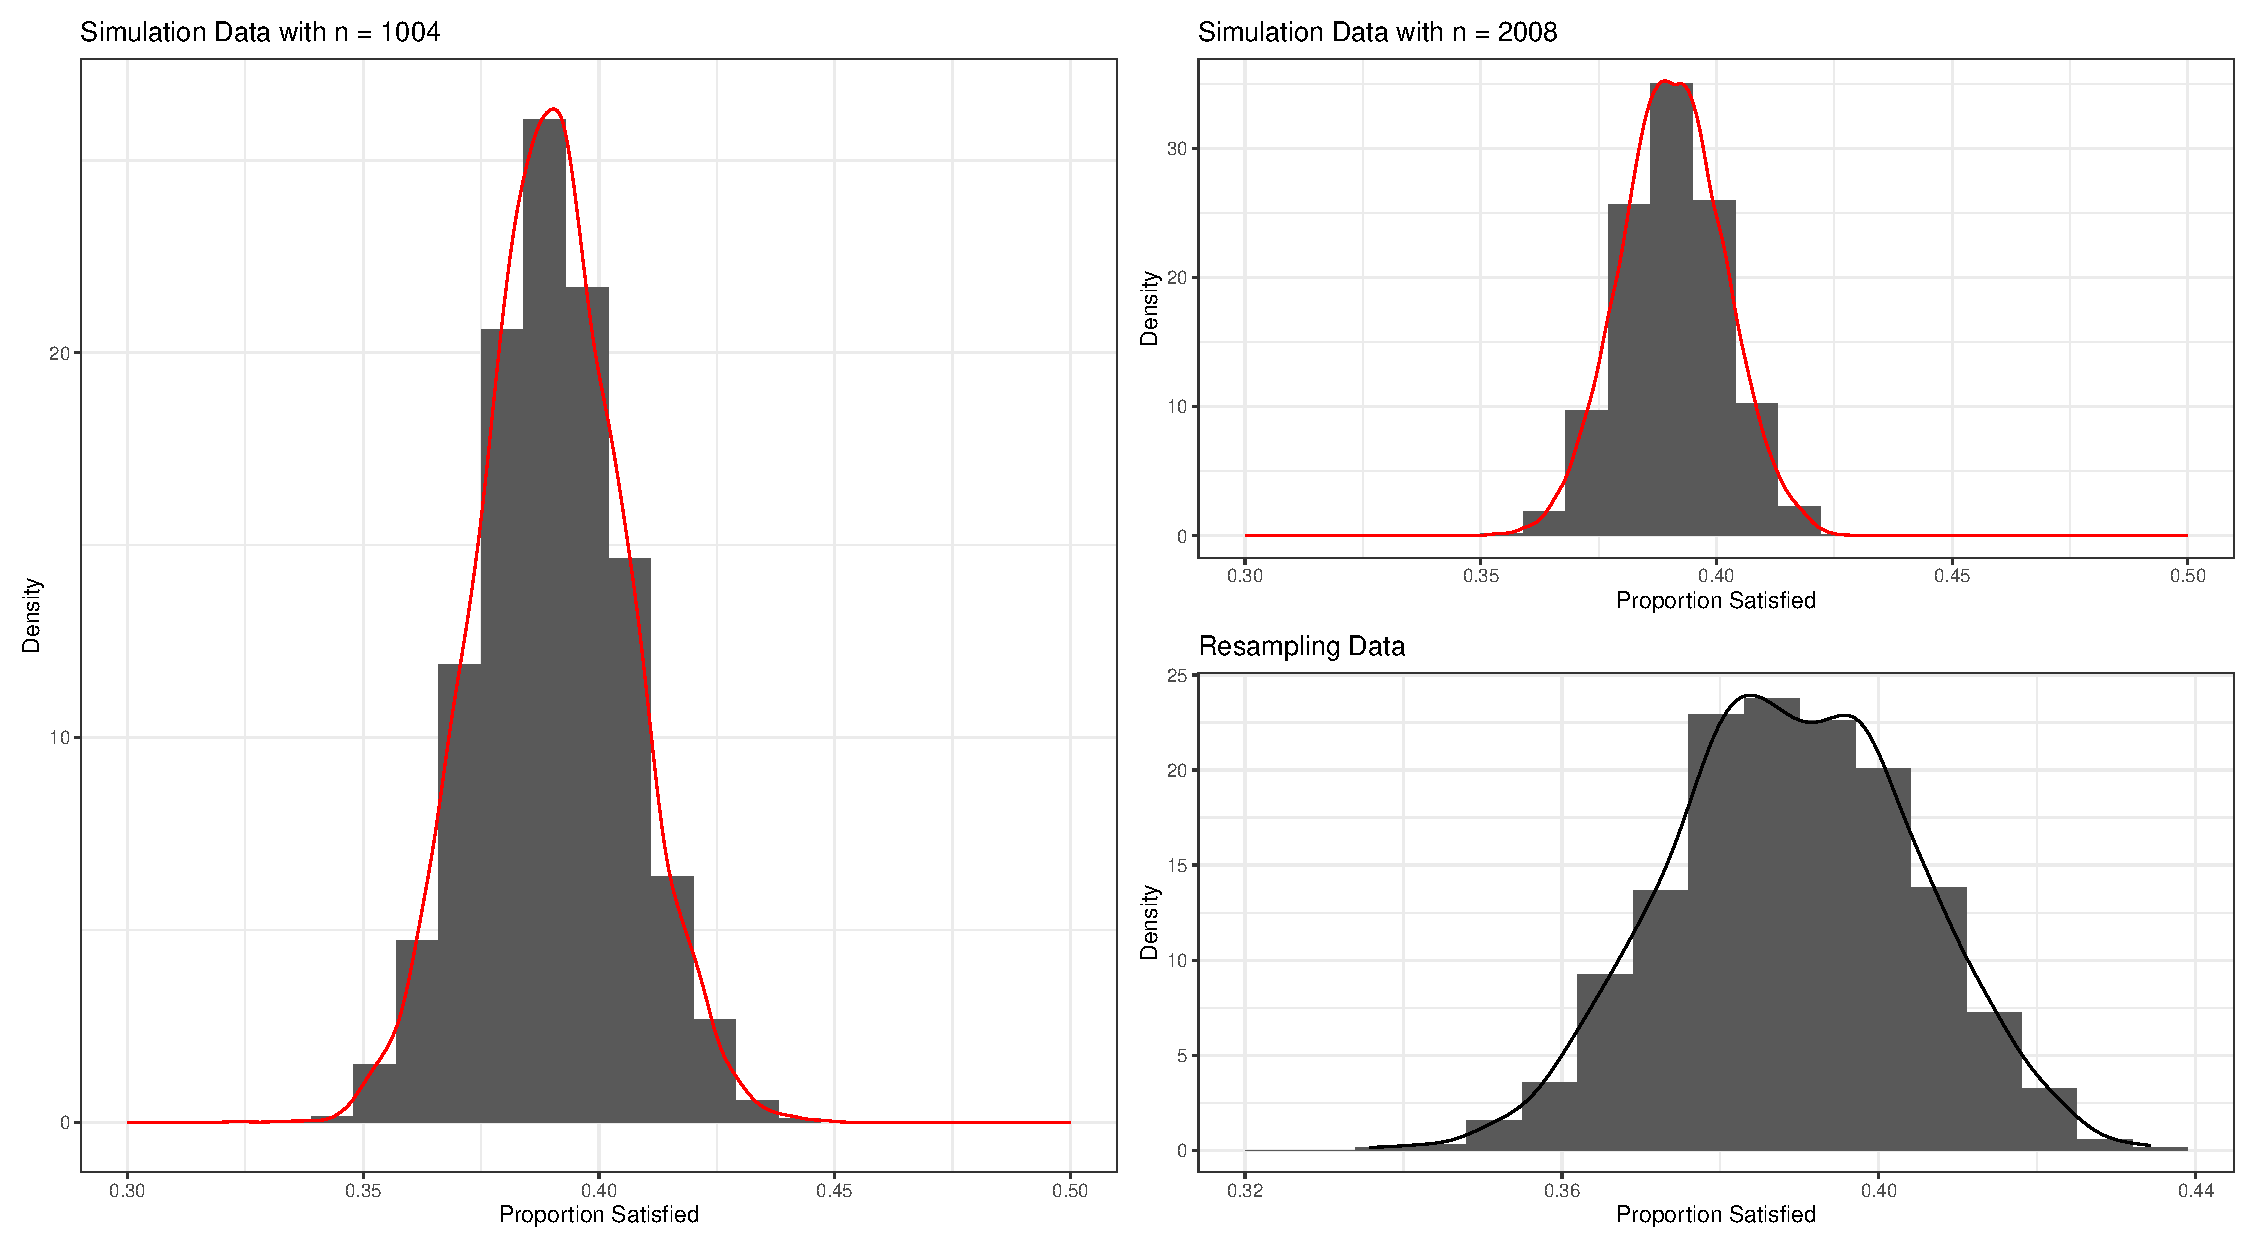
\includegraphics[scale=0.35]{graphs.pdf}
    \caption{}
    \label{moe}
  \end{center}
\end{figure}

\begin{figure}[H]
  \begin{center}
    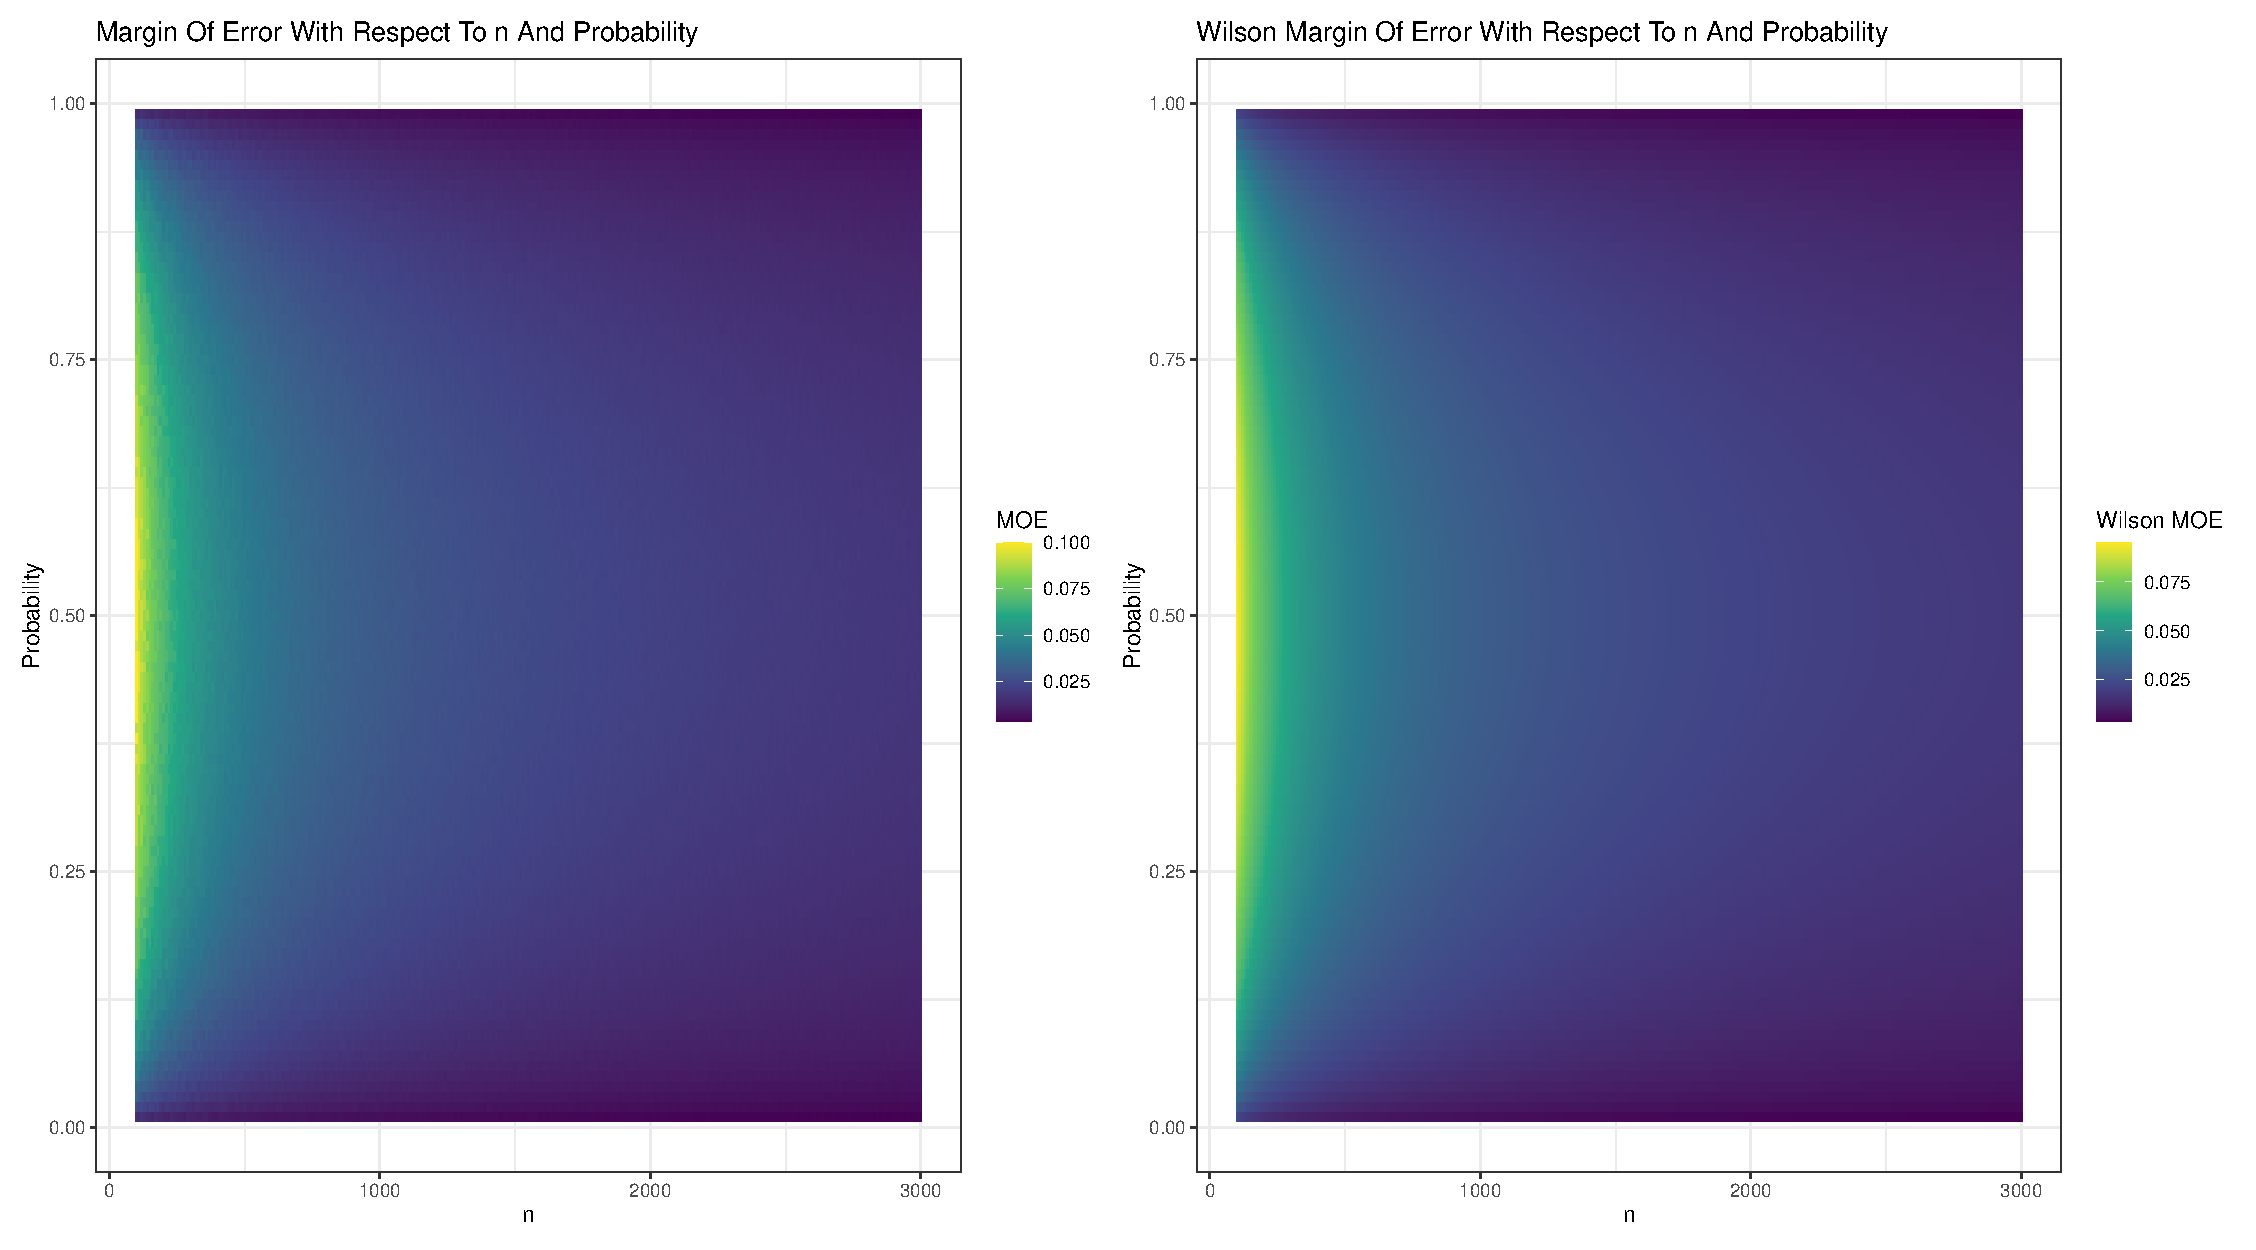
\includegraphics[scale=0.35]{raster.pdf}
    \caption{}
    \label{moe}
  \end{center}
\end{figure}

\end{document}
